\section{Diseño e Implementación}\label{sec:design}

Para la realización del proyecto se decidió implementar un SRI vectorial. Se
utilizó TF-IDF (\emph{Term Frecuency - Inverse Document Frequency} por sus
siglas en inglés) como base principal de los modelos por la sencillez de su
implementación y el gran potencial que ofrece.

Para analizar el diseño de la aplicación se realizará una descripción de forma
\emph{top-down}. Primero se mostrarán las capas superiores comenzando por la
interacción del usuario con la aplicación y luego se analizará de forma
detallada el diseño e implementación de cada una de las componentes que
conforman la misma.

De forma general el usuario tiene dos formas de interactuar con la aplicación:
mediante una interfaz de lineas de comando en una terminal (\emph{Command Line
Interface}, CLI por sus siglas en inglés) desarrollada usando \emph{typer} o
mediante una interfaz gráfica desarrollada usando \emph{streamlit} (ambas
lbrerías de Python).

Para hacer uso de la aplicación y comenzar a realizar consultas a una base de
datos, el usuario debe realizar primero dos acciones:

\begin{enumerate}
	\item Construir la base de datos.
	\item Construir el modelo de RI de la base de datos construida.
\end{enumerate}

Luego de ello, el usuario puede realizar consultas a la base de datos o
evaluar el modelo de RI de alguna de las bases de datos ya integradas. En
la figura \ref{fig:interaction} se muestra un simple esquema de la
interacción con la aplicación.

\begin{figure}[htb]%
	\begin{center}
		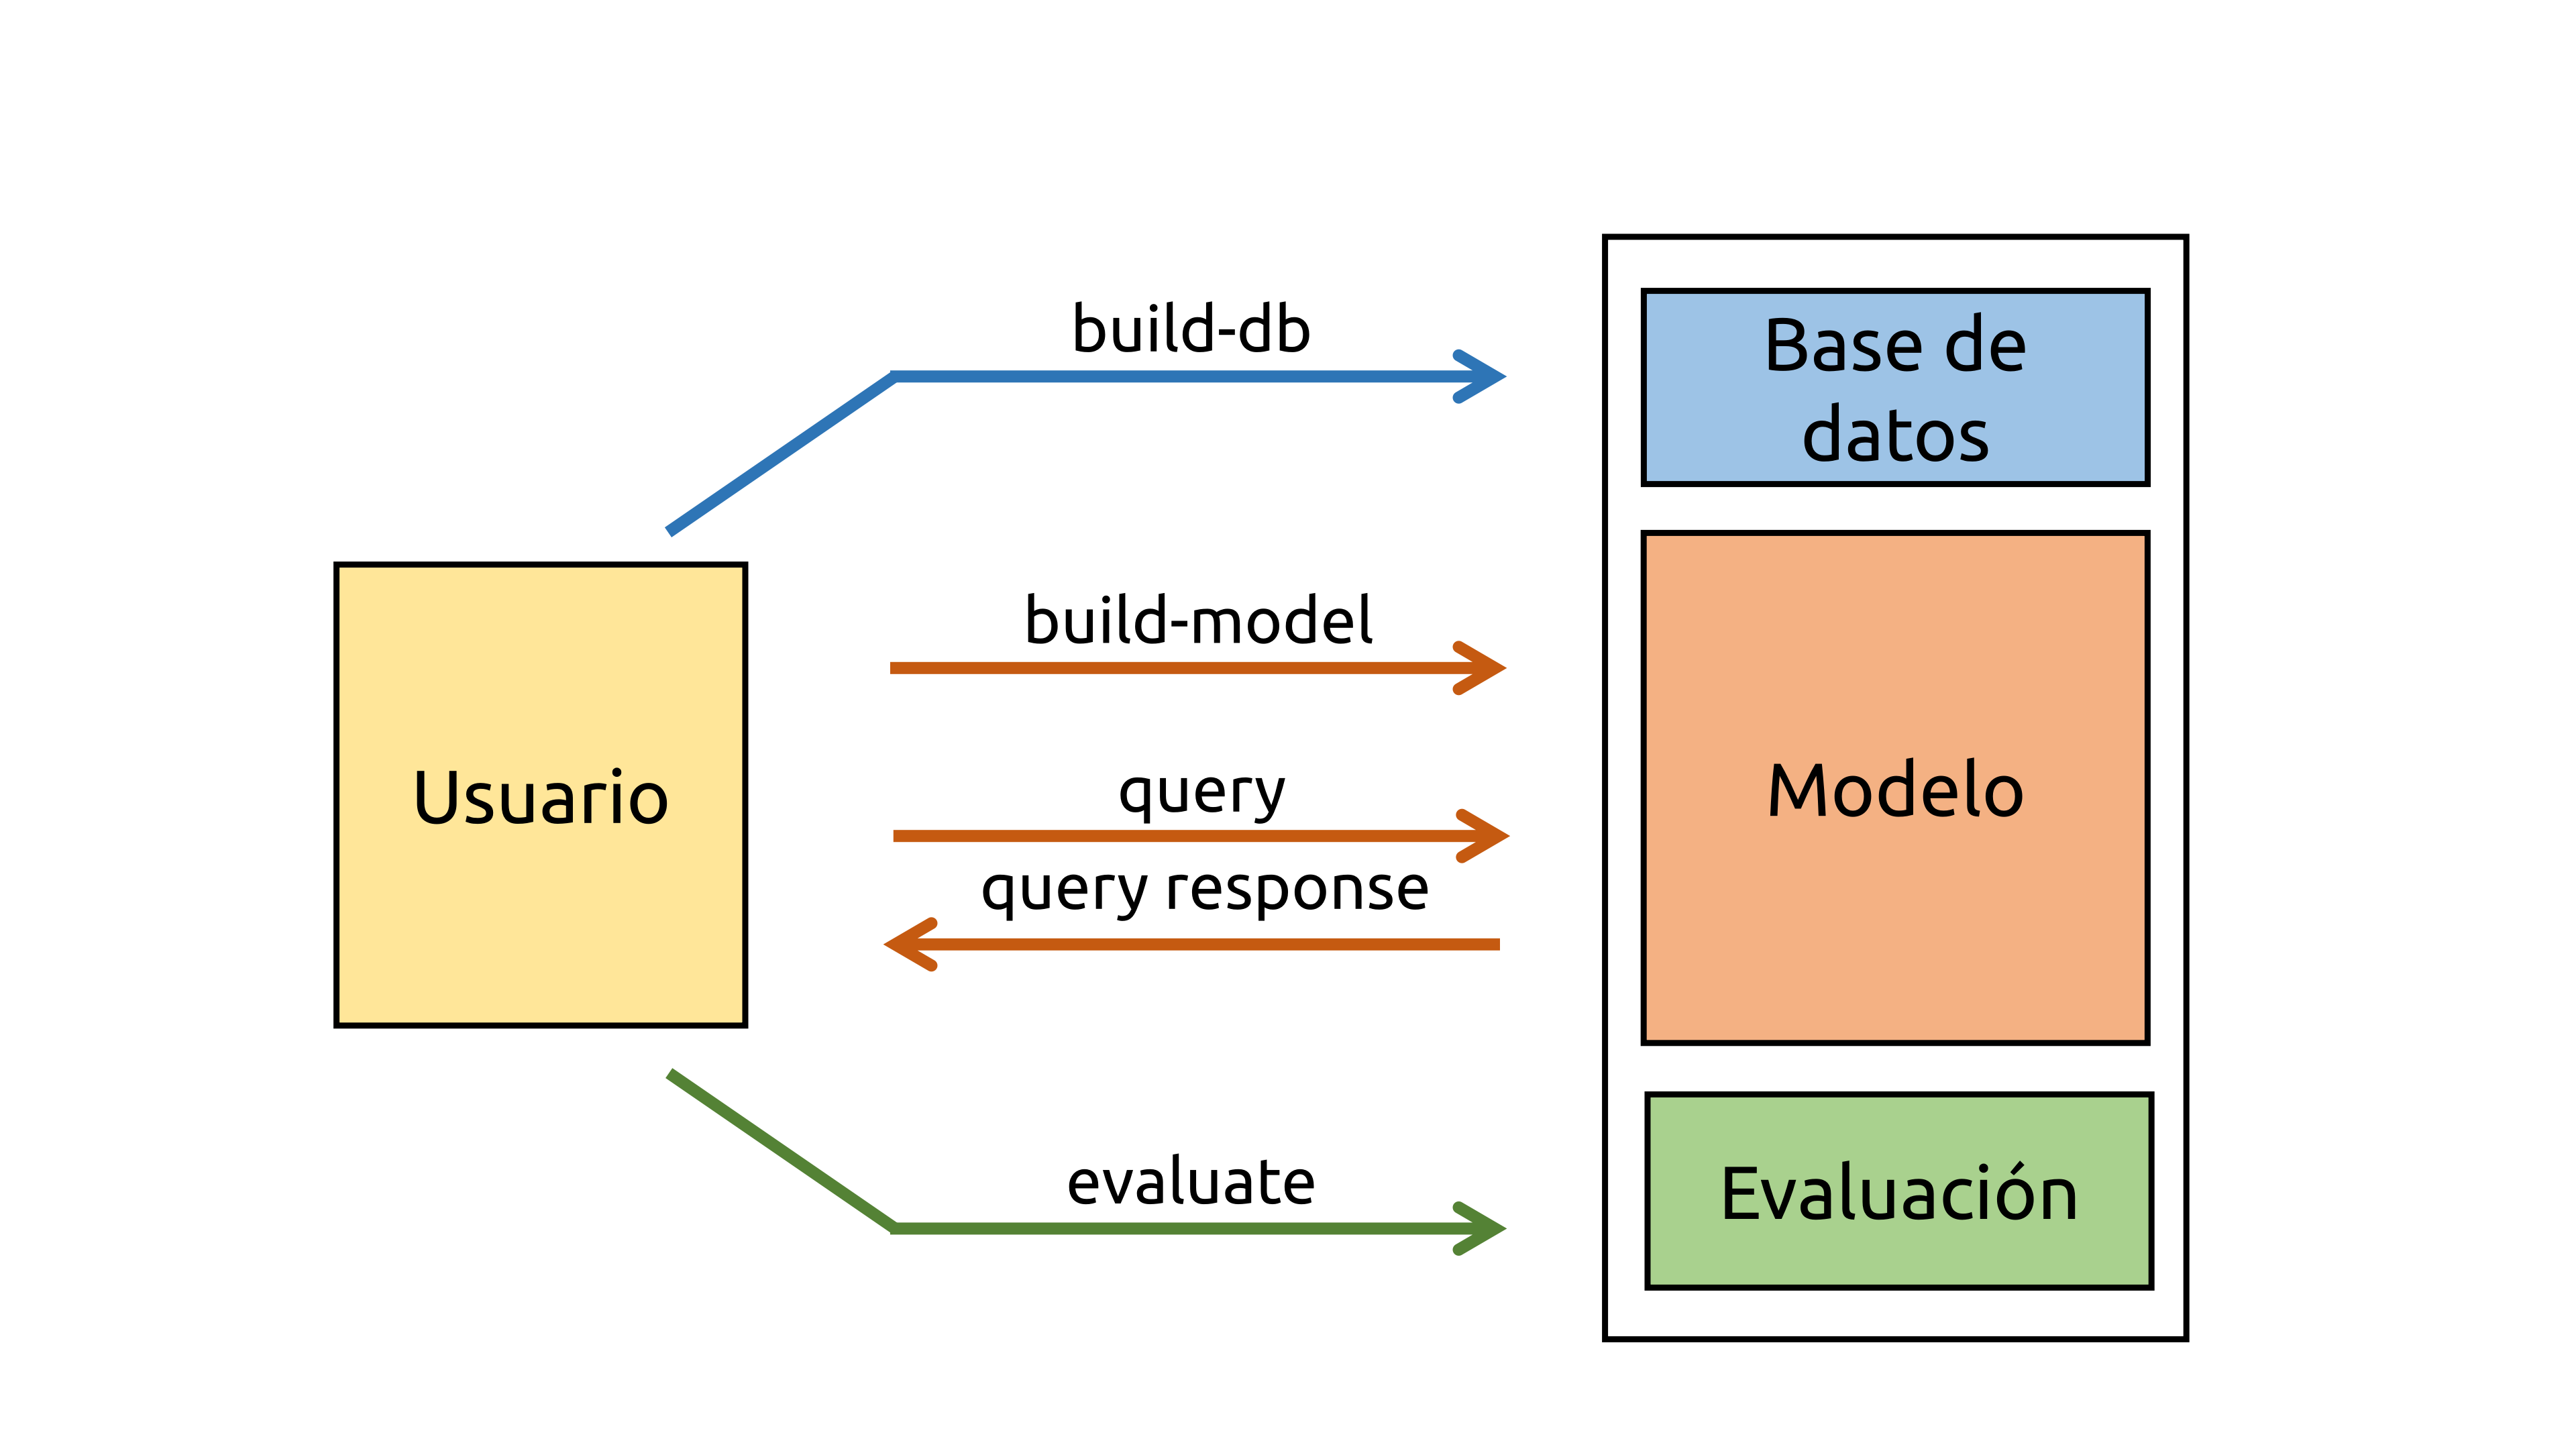
\includegraphics[width=0.8\textwidth]{./sri_01.png}
	\end{center}
	\caption{Esquema general de interacción del usuario con Switer}
	\label{fig:interaction}
\end{figure}

\subsection{Estructura de la base de datos}\label{sec:build-database}

Una base de datos en la aplicación está constituida por dos archivos:
\emph{docs.json} y \emph{metadata.json}. El primero representa
una lista donde cada posición contiene el texto de un documento. El
segundo archivo contiene una lista de diccionarios donde cada uno
contiene los metadatos del documento de mísmo índice.

\subsection{Modelos}\label{sec:model}

El modelo de una base de datos se construye de acuerdo a los paramentros de
configuración. Estos parametros son:

\begin{itemize}
	\item \textbf{tokenization\_method}: Método de tokenización de los
		documentos. Puede ser \emph{split} o \emph{nltk}. En caso de ser
		\emph{split} su usará la función \emph{split} de Python y se
		dividirá el texto solo por espacios. En caso de ser \emph{nltk} se
		usará la función \emph{word\_tokenize} de NLTK.
	\item \textbf{include\_metadata}: Una lista con los nombres de los
		metadatos que se desean incluir en el texto para construir el modelo.
	\item \textbf{query\_alpha\_smoothing}: Valor del parámetro $\alpha$ usado
		para suavisar el vector de la consulta.
	\item \textbf{remove\_stopwords}: Si es \emph{true} se eliminarán las
		palabras comunes (proporcionadas por \emph{nltk}).
	\item \textbf{remove\_punctuation}: Si es \emph{true} se eliminarán los
		puntuaciones.
	\item \textbf{lemmatization}: Si es \emph{true} se lematizarán las
		palabras. Esto significa que se tendrá en cuenta la palabra origen de
		cada vocablo. Por ejemplo, si se lematizan la palabras \emph{playing,
		played, etc} se tendrá en cuenta la palabra \emph{play} que es la
		palabra origen de \emph{playing}.
	\item \textbf{stemming}: Si es \emph{true} se agregará también la raíz de
		cada palabra al documento. Esto es difere de la lematización en que
		la palabra resultante no tiene por qué ser una palabra real en sí. Por
		ejemplo, si se aplica semming a las palabras \emph{change, changing,
		changed, etc} se puede obtener la palabra \emph{chang}.
\end{itemize}

Como se puede observar la mayoria de los parámetros están relacionados
con el proceso de tokenización de los documentos, ya que esta es una de las
operaciones más importantes para construir el modelo.

La figura \ref{fig:model-build} muestra un esquema del proceso de construcción del
modelo.

\begin{figure}[htb]%
	\begin{center}
		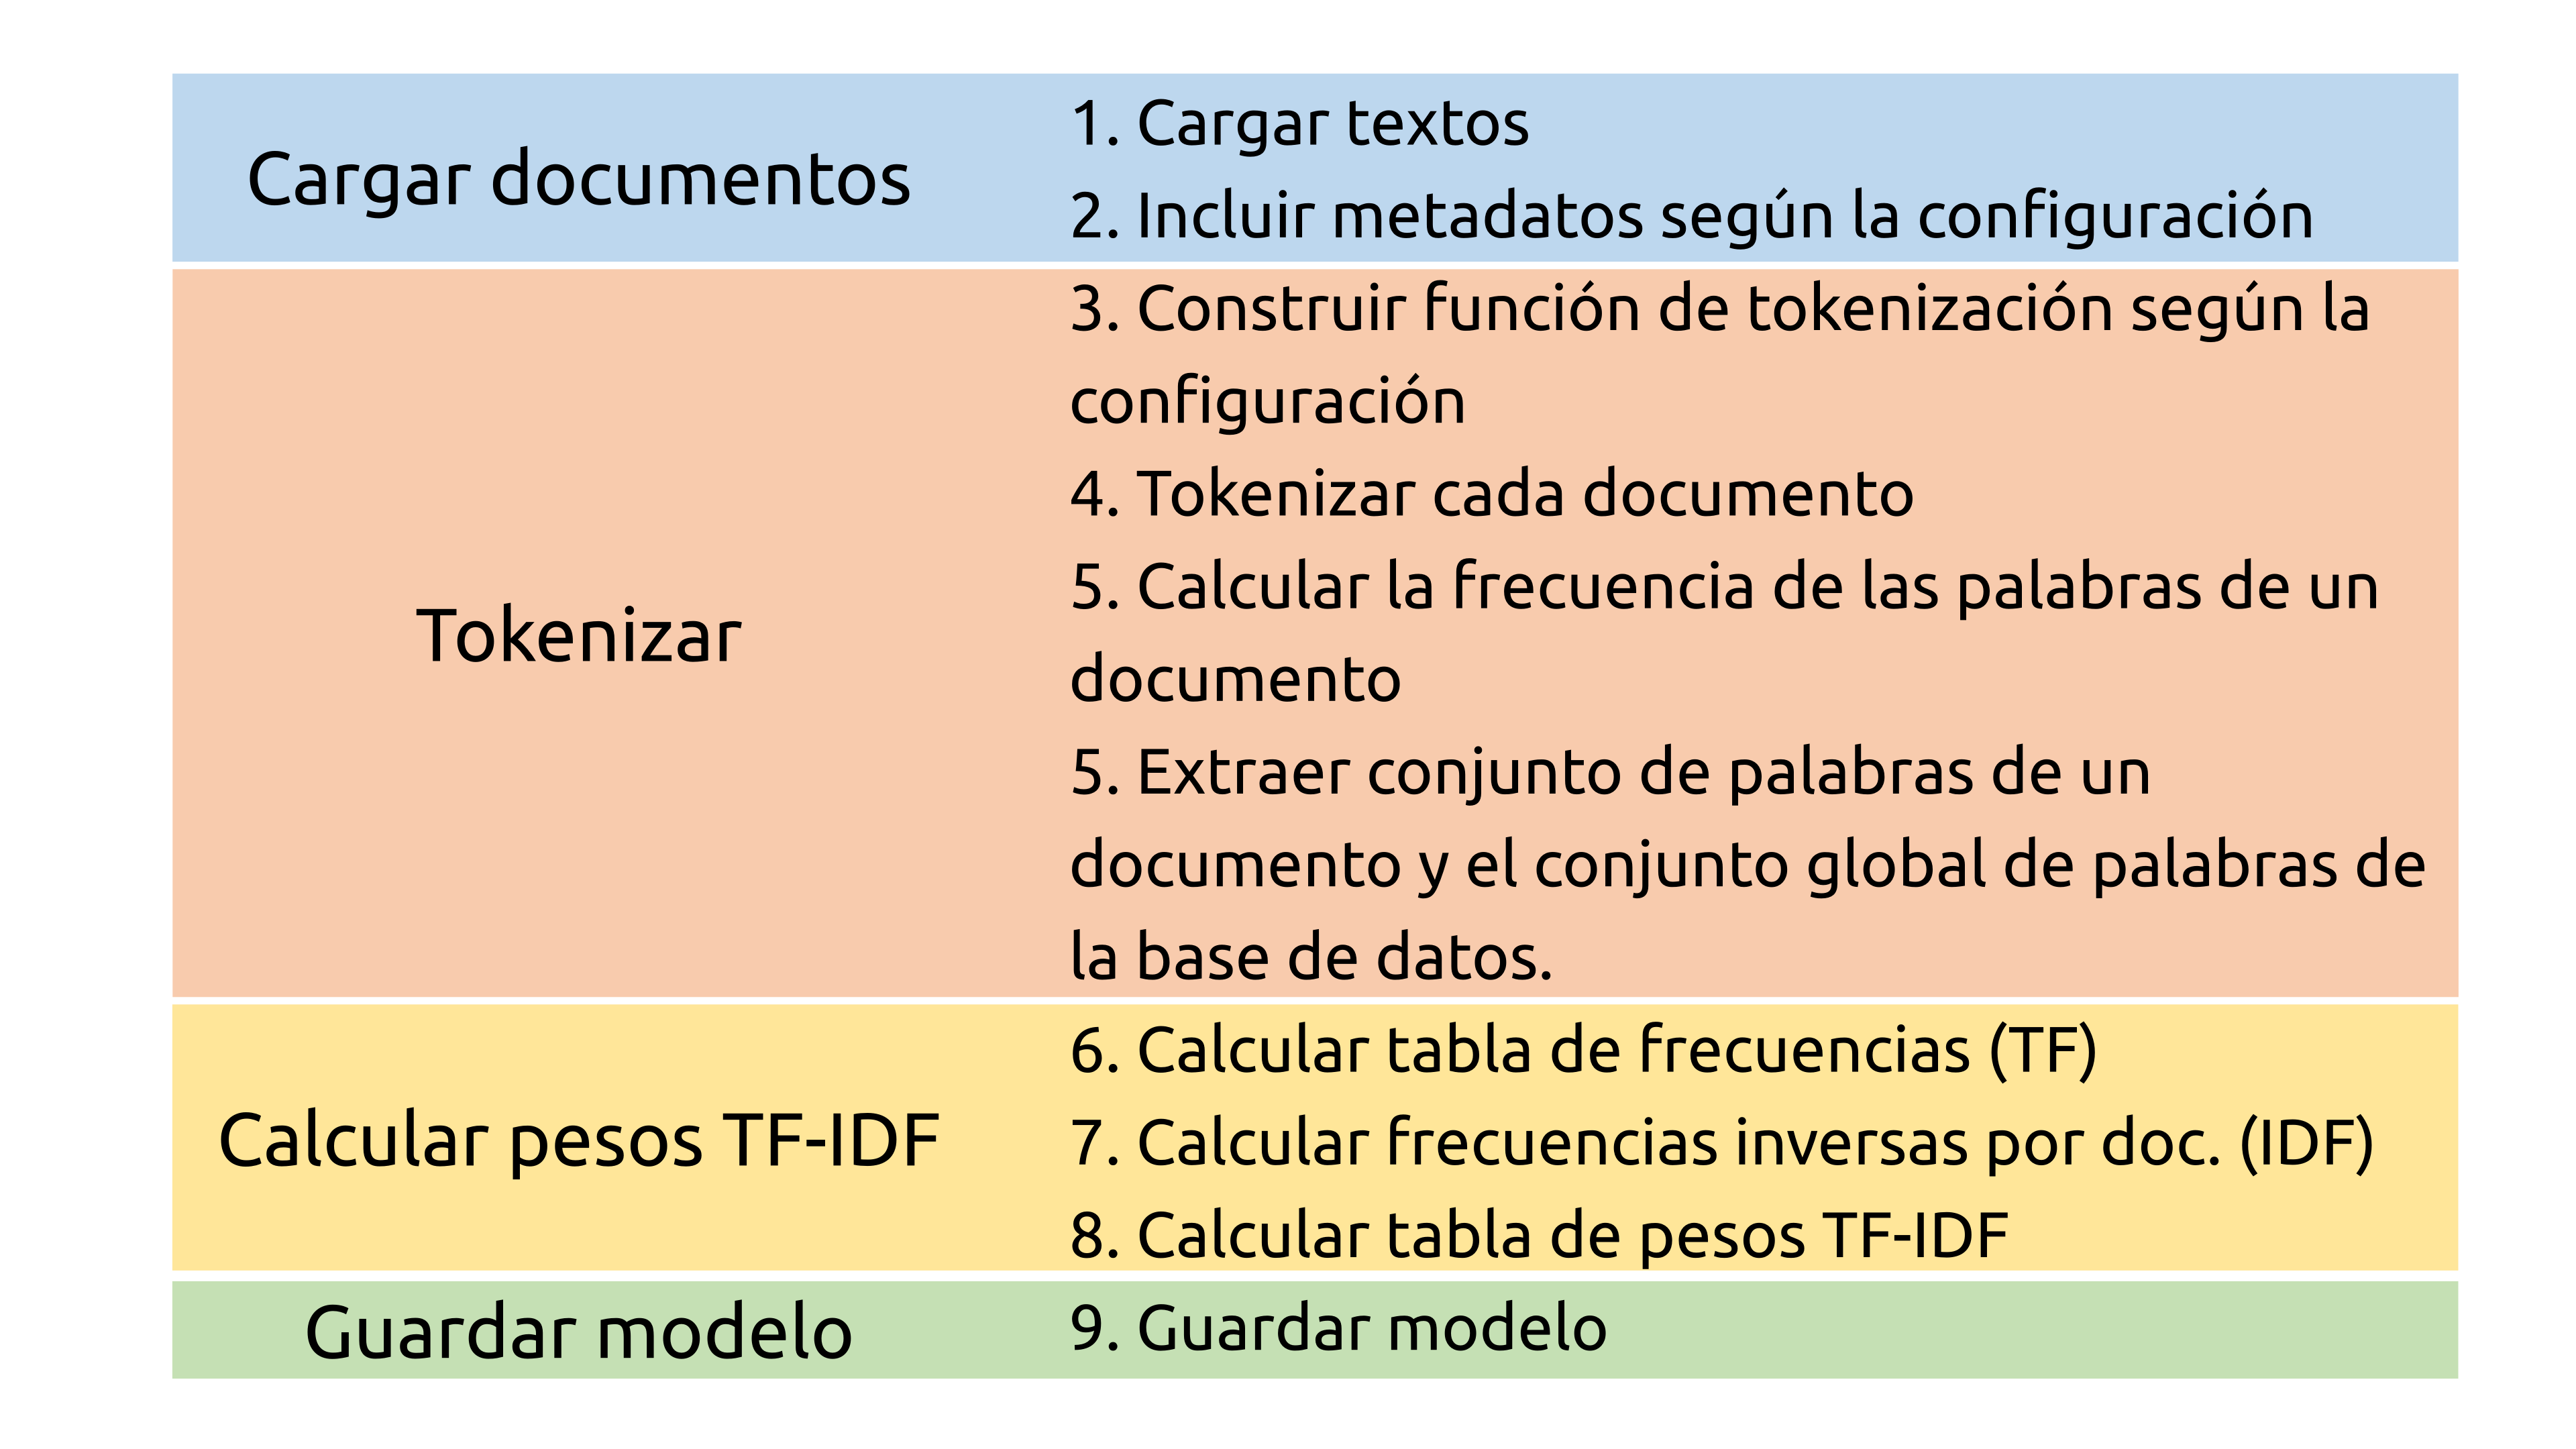
\includegraphics[width=0.8\textwidth]{./sri_02.png}
	\end{center}
	\caption{Construcción de un modelo}
	\label{fig:model-build}
\end{figure}

Primeramente se cargan los textos del archivo \emph{docs.json} de la base de
datos. A cada texto se le agrega según la configuración los metadatos necesarios.

Luego se procede a la construcción de la función que tokeniza cada documento.
Esta función se construye en base a los parametros establecidos en el archivo
de configuración. Una vez contruida, se extraen los las palabras (tokens) de
cada docuemnto y se calcula la frecuencia de cada una de ellas por cada uno de
los textos. Posteriormente se construye el vocabulario del modelo con el
conjunto de todas las palabras.

Con la información de las frecuencias se crea la tabla de frecuencia de palabra
por documento y se normaliza (\emph{term frecuency} o TF). Se calcula además el
vector de frecuencia inversa por documento (\emph{inverse document frequency} o
IDF). Luego se construye la tabla TF-IDF con los datos anteriores.

Finalmente, se almacena la tabla TF-IDF junto con información adicional del modelo
como: \emph{id} (un identificador único), fecha y duración de la construcción, así
como la configuración usada.

Cada base de datos contiene un único modelo, esto permite al usuario realizar
diferentes modelos con diferentes configuraciones según la base de datos.

\subsection{Consultas}\label{sec:query}

Una vez construido el modelo, el usuario puede realizar consultas a la base de
datos. Para ello, solo basta con especificar la base de datos que se quiere
consultar y la consulta que se desea realizar. 

Para procesar la consulta se utiliza la misma función de tokenización que se
utilizó para construir el modelo. Las palabras que no estén en el vocabulario
son ignoradas. Se calcula el vector de consulta y luego utilizando la operación
de coseno entre vectores se calcula la relevancia de cada documento con
respecto a la consulta. Una vez calculada las relevancias, se organiza los
documentos de mayor a menor según este valor y se devuelven en este orden.

En el caso del CLI proporcionado los documentos se van devolviendo uno a uno
y en cada momento el usuario puede especificar si quiere ver el siguiente
documento o no. En la aplicación web desarrollada con \emph{streamlit} en cada
consulta el usuario puede establecer un numero máximo de documentos a mostrar
y un peso de relevancia mínimo para los resultados.

Cada resultado contiene el texo del documento, sus metadatos y la relevancia 
obtenida de acuerdo a la consulta realizada.

\subsection{Código}\label{sec:code}

El proyecto está implementado completamente en Python, por ser este un lenguaje
de programación fácil de usar y con una gran cantidad de funcionalidades. Además
de la gran variedad de librerías existentes para el prosesamiento de texto y
desarrollo de apliaciones.

Para lograr una mejor integración del código con las diferentes aplicaciones
implementadas (CLI y aplicación web) se implementaron las funciones principales
en un módulo que funciona como API (\emph{Aplication Programming Interface} por sus
siglas en inglés). Las aplicaciones con las que el usuario interactúa se
comunincan con el API, esta a su vez realiza las operaciones necesarias en las
bases de datos y modelos, y luego devuelve los resultados a la aplicación que
esté usando el usuario. En la figura \ref{fig:project-structure} se muestra un
esquema de la estructura del proyecto.

\begin{figure}[htb]%
	\begin{center}
		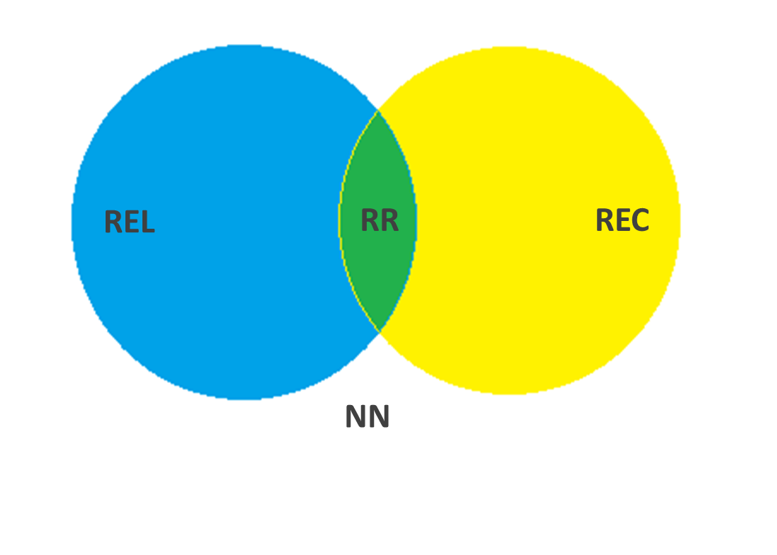
\includegraphics[width=0.8\textwidth]{./sri_03.png}
	\end{center}
	\caption{Estructura del proyecto}
	\label{fig:project-structure}
\end{figure}

Para mejorar la eficiencia del API cada modelo, así como los resultados de cada
evaluación del mismo, se guardan junto con la base de datos. De esta forma el 
modelo solo se construye una vez y se puede utilizar en cualquier aplicación
que requiera realizar consultas sobre el mismo. Por ello, muchas de las funciones
del API poseen un parámetro \emph{force} que permite forzar la ejecución de
comandos a pesar de que exista la información ya guardada.

Se ofrece a los usuarios desarrolladores una estructura \emph{DatabaseBuilder}.
Esta clase se encarga de crear una nueva base de datos dado una lista de textos
(documentos) y una lista de diccionarios del mismo tamaño (metadatos). De
esta forma se le evita al desarrollador la tarea de crear las carpetas y archivos
de la forma que el API las consume.

De forma integrada en el proyecto se ofrecen tres bases de datos: \emph{Cranfield},
\emph{Medline} y \emph{CISI}. Los modelos de cada una pueden ser sometidos a 
evaluación.

\subsubsection{Herramientas externas usadas}\label{sec:external-tools}

Como se mencionó anteriormente, para la creación del CLI y la aplicación web se
usaron las librerías \emph{typer} y \emph{streamlit} respectivamente. En el
proceso de consteucción de los modelos se utilizó la librería \emph{nltk} para
el tokenizado de textos y en la utilización de algunos recursos como un
conjunto de palabras comunes del idioma inglés. Para la visualización de los
resultados se utilizó la librería \emph{matplotlib}.
